\documentclass{standalone}
\usepackage{tikz}
\usepackage{ctex,siunitx}
\setCJKmainfont{Noto Serif CJK SC}
\usepackage{tkz-euclide}
\usepackage{amsmath}
\usetikzlibrary{patterns, calc,3d}
\usetikzlibrary {decorations.pathmorphing,decorations.pathreplacing,decorations.shapes}
\begin{document}
\small
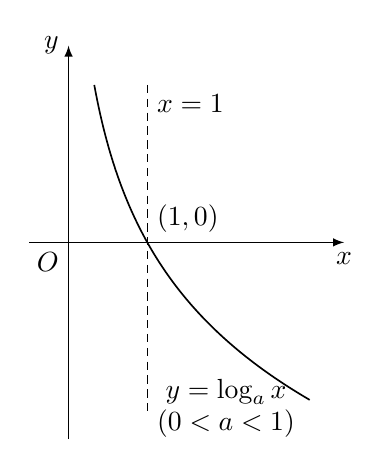
\begin{tikzpicture}[>=latex,scale=1.0]
  \draw[->](-0.5,0)--(3.5,0)node[below]{$x$};
  \draw[->](0,-2.5)--(0,2.5)node[left]{$y$};
  \node at (0,0)[below left]{$O$};
  \draw[densely dashed](1,2.0)node[below right]{$x=1$}--(1,-2.2);
  \draw[semithick,samples=200,domain=-2:2]plot({pow(4/7,\x)},\x);
  \node at (2.0,-2.3){$(0<a<1)$};
  \node at (2.0,-1.9){$y=\log_ax$};
  \node at (1,0)[above right]{$(1,0)$};
\end{tikzpicture}
\end{document}